\documentclass[12pt]{article}

\usepackage{mathpazo}
\usepackage[a4paper, landscape, margin=10mm]{geometry}
\usepackage[utf8]{inputenc}
\usepackage[table]{xcolor}
\usepackage{icomma}
\usepackage{graphicx}
\usepackage{multicol}
\usepackage{textcomp}

\begin{document}

\thispagestyle{empty}
\centering
\begin{center}
{\LARGE \bfseries LOM3226 --- 1\textordmasculine{} semestre de 2023}\\[4mm] 
{\Large \bfseries Resultado Final} 
\end{center} 
\vfill
\begin{multicols}{2}
\centering 
\rowcolors{2}{gray!25}{white} 
\begin{tabular}{lccc} 
\hline 
\rowcolor{gray!50}\textbf{NUSP} & \textbf{P1} & \textbf{P2} & \textbf{NF} \\ 
\hline 
1 & \textcolor{red}{3,2} & \textcolor{blue}{5,2} & \textcolor{blue}{5,0} \\ 
2 & \textcolor{red}{4,2} & \textcolor{red}{3,1} & \textcolor{blue}{5,0} \\ 
3 & \textcolor{blue}{9,9} & \textcolor{blue}{10,0} & \textcolor{blue}{9,6} \\ 
4 & \textcolor{blue}{7,3} & \textcolor{blue}{10,0} & \textcolor{blue}{8,3} \\ 
5 & \textcolor{blue}{6,5} & \textcolor{red}{1,5} & \textcolor{red}{4,1} \\ 
6 & \textcolor{blue}{8,0} & \textcolor{blue}{10,0} & \textcolor{blue}{8,0} \\ 
7 & \textcolor{blue}{9,5} & \textcolor{blue}{10,0} & \textcolor{blue}{9,4} \\ 
8 & \textcolor{blue}{7,0} & \textcolor{blue}{9,5} & \textcolor{blue}{6,7} \\ 
9 & \textcolor{red}{1,5} & \textcolor{blue}{7,5} & \textcolor{red}{4,2} \\ 
10 & \textcolor{red}{3,4} & \textcolor{blue}{10,0} & \textcolor{blue}{6,1} \\ 
11 & \textcolor{blue}{7,6} & \textcolor{blue}{7,2} & \textcolor{blue}{7,2} \\ 
12 & \textcolor{red}{0,0} & \textcolor{blue}{5,5} & \textcolor{blue}{5,1} \\ 
13 & \textcolor{blue}{5,7} & \textcolor{blue}{9,3} & \textcolor{blue}{6,2} \\ 
14 & \textcolor{blue}{7,8} & \textcolor{blue}{7,5} & \textcolor{blue}{5,3} \\ 
15 & \textcolor{red}{4,8} & \textcolor{blue}{9,0} & \textcolor{blue}{5,4} \\ 
16 & \textcolor{red}{4,0} & \textcolor{blue}{6,3} & \textcolor{blue}{5,8} \\ 
17 & \textcolor{blue}{5,9} & \textcolor{blue}{8,2} & \textcolor{blue}{6,0} \\ 
18 & \textcolor{blue}{7,4} & \textcolor{blue}{10,0} & \textcolor{blue}{7,1} \\ 
19 & \textcolor{blue}{9,5} & \textcolor{blue}{10,0} & \textcolor{blue}{8,4} \\ 
20 & \textcolor{red}{1,8} & \textcolor{blue}{7,5} & \textcolor{blue}{5,1} \\ 

\hline 
\end{tabular} 

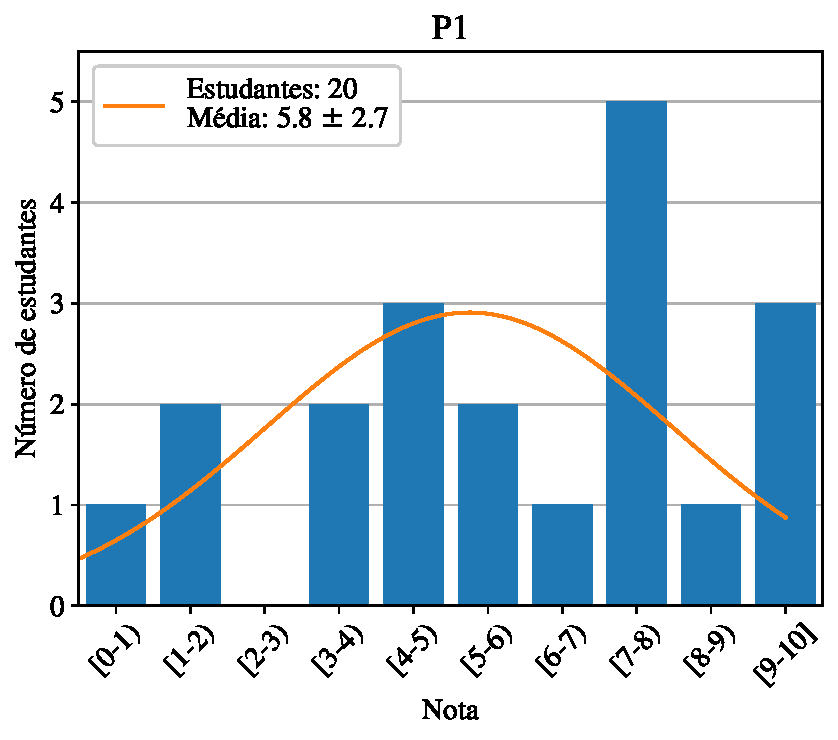
\includegraphics[width=\columnwidth]{hist-P1.pdf}
\begin{minipage}{\columnwidth}
\begin{flushright}
Azuis: 12

Vermelhas: 8 
\end{flushright}
\vskip 5mm
\end{minipage}
\end{multicols}

\end{document}
